\documentclass[a4paper,oneside,11pt]{book}
\usepackage{tikz}
\usetikzlibrary{arrows}
\usepackage{graphicx}
\usepackage{titling}
\usepackage{geometry}
\usepackage{listings}
\usepackage{xcolor}
\usepackage{float}
\usepackage{hyperref}
\usepackage{indentfirst}
\usepackage{titlesec}
\usepackage{booktabs}
\usepackage{amsmath}
\usepackage{amssymb}
\usepackage{amsfonts}
\usepackage{array}
\usepackage{multirow}

% Pengaturan margin standar UGM (Kiri 3cm, Kanan 2.5cm, Atas 3cm, Bawah 3cm)
\geometry{
    left=3cm,
    right=2.5cm,
    top=3cm,
    bottom=3cm
}

% Pengaturan warna untuk kode
\definecolor{codegreen}{rgb}{0,0.6,0}
\definecolor{codegray}{rgb}{0.5,0.5,0.5}
\definecolor{codepurple}{rgb}{0.58,0,0.82}
\definecolor{backcolour}{rgb}{0.96,0.96,0.94}
\definecolor{codeblue}{rgb}{0,0,0.7}
\definecolor{darkgray}{rgb}{0.2,0.2,0.2}

% Style listings umum
\lstdefinestyle{codestyle}{
    backgroundcolor=\color{backcolour},   
    commentstyle=\color{codegreen},
    keywordstyle=\color{codepurple}\bfseries,
    numberstyle=\tiny\color{codegray},
    stringstyle=\color{codeblue},
    basicstyle=\ttfamily\footnotesize,
    breakatwhitespace=false,         
    breaklines=true,                 
    captionpos=b,                    
    keepspaces=true,                 
    numbers=left,                    
    numbersep=5pt,                  
    showspaces=false,                
    showstringspaces=false,
    showtabs=false,                  
    tabsize=2,
    frame=single
}

\lstdefinestyle{outstyle}{
    backgroundcolor=\color{white},
    basicstyle=\ttfamily\scriptsize,
    breakatwhitespace=false,
    breaklines=true,
    keepspaces=true,
    showspaces=false,
    showstringspaces=false,
    showtabs=false,
    frame=single
}

\lstset{style=codestyle}

\titleformat{\chapter}[hang]
{\bfseries\LARGE}
{\LARGE\thechapter.}{1em}{}
\titlespacing*{\chapter}{0pt}{0pt}{15pt}

\hypersetup{
    colorlinks=true,
    linkcolor=black,
    filecolor=magenta,      
    urlcolor=blue,
    citecolor=blue
}

\begin{document}

% ==================== HALAMAN JUDUL (COVER) ====================
\begin{titlepage}
\centering

\vspace*{0.2cm}

{\LARGE \textbf{LAPORAN UJIAN TENGAH SEMESTER}}\\[0.8cm]
{\Large \textbf{Konstruksi dan Evolusi Perangkat Lunak}}\\[0.4cm]
{\large Kode MK: SVPL261501 (2 SKS)}\\[1.2cm]

{\Large \textbf{TAHUN AKADEMIK GASAL 2026/2027}}\\[0.6cm]

{\large \textbf{ARSITEKTUR CLIENT-SERVER RESTFUL API LARAVEL DENGAN SANCTUM, FRONTEND VUE.JS, DOCKER COMPOSE, DAN CI/CD PIPELINE}}\\[0.3cm]
{\normalsize Tema: Sistem Inventaris Peralatan Produksi Multimedia \& Perangkat Studio}\\[1.5cm]


\includegraphics[height=6.5cm]{lambang ugm.png}\\[1.5cm]

{\large 
\textbf{Nama Mahasiswa :} Muhammad Abel Abhinaya Riananto\\
\textbf{NIM / NIU        :} 24/544597/SV/25468 (544597)\\
\textbf{Program Studi    :} D4 Teknologi Rekayasa Perangkat Lunak\\
\textbf{Departemen       :} Teknik Elektro dan Informatika\\
\textbf{Fakultas         :} Sekolah Vokasi\\
\textbf{Universitas      :} Universitas Gadjah Mada
}\\[1.0cm]

{\large 
\textbf{Dosen Pengampu:}\\
Dr. Muhammad Fakhrurrifqi, S.Kom., M.Cs.\\
Galih Malela Damaraji, S.Pd., M.Eng.
}

\vfill
Yogyakarta, 15 Oktober 2026

\end{titlepage}

% ==================== DAFTAR ISI ====================
\tableofcontents
\newpage

% ==================== BAB 1 ====================
\chapter{Tujuan Ujian Tengah Semester}

Pelaksanaan Ujian Tengah Semester mata kuliah Konstruksi dan Evolusi Perangkat Lunak (SVPL261501) ini bertujuan untuk menguji dan mengevaluasi Capaian Pembelajaran Mata Kuliah (CPMK) mahasiswa secara terpadu melalui pembangunan sistem nyata berbasis standar industri perangkat lunak modern:
\begin{enumerate}
\item \textbf{CPMK 1 (Konsep Dasar DevOps dan Filosofi Agile)}: Mampu merancang dan mengimplementasikan arsitektur \textit{client-server} yang terpisah secara murni (\textit{decoupled architecture}), di mana backend Laravel menyediakan RESTful API berbasis JSON dengan autentikasi token (Laravel Sanctum), dan frontend Vue.js mengonsumsi data secara dinamis melalui pustaka Axios.
\item \textbf{CPMK 2 (Continuous Integration dan Manajemen Repositori GitHub)}: Mampu mengelola siklus hidup kode sumber menggunakan sistem kendali versi Git dengan strategi pencabangan terstruktur (\textit{branching model}: \texttt{main}, \texttt{dev}, dan \texttt{feature/*}), menerapkan kebijakan perlindungan cabang (\textit{branch protection rules}) dengan kewajiban Pull Request dan \textit{status check}, serta menyusun alur kerja otomatisasi pengujian (\textit{CI Pipeline}) menggunakan GitHub Actions.
\item \textbf{CPMK 3 (Continuous Deployment untuk Laravel)}: Mampu merancang alur penerapan otomatis (\textit{Continuous Deployment}) berbasis kondisi cabang, mengamankan nilai rahasia produksi (\textit{secrets}) menggunakan GitHub Secrets, dan mengunggah artefak kontainer Docker ke \textit{registry} terdistribusi (\textit{GitHub Container Registry} / GHCR) dengan penandaan (\textit{tagging}) berbasis nomor \textit{commit SHA}.
\item \textbf{CPMK 4 \& CPMK 5 (Docker dan Konsep Containerization)}: Mampu menyusun berkas instruksi kontainerisasi (\texttt{Dockerfile}) untuk backend dan frontend dengan memanfaatkan prinsip \textit{multi-stage build}, mengoptimalkan waktu kompilasi melalui \textit{Docker layer caching}, mengonfigurasi berkas eliminasi \texttt{.dockerignore}, serta mencegah kebocoran informasi kredensial di dalam citra kontainer.
\item \textbf{CPMK 6 \& CPMK 7 (Docker Compose dan Deployment Berbasis Kontainer)}: Mampu mengorkestrasikan sistem \textit{multi-container} (\textit{database}, backend, dan frontend) melalui berkas \texttt{docker-compose.yml} dengan satu perintah eksekusi (\texttt{docker compose up -d --build}), menghubungkan layanan melalui \textit{service discovery} pada jaringan internal Docker bridge, serta memastikan persistensi data relasional menggunakan \textit{named volume}.
\item \textbf{Nilai Tambahan (+10 Poin)}: Mampu mengoperasikan backend Laravel menggunakan server aplikasi generasi baru berbasis bahasa Go, yaitu \textbf{FrankenPHP} (ditenagai mesin Caddy Server), menggantikan server web konvensional PHP-FPM / Nginx atau \texttt{php artisan serve}.
\end{enumerate}

% ==================== BAB 2 ====================
\chapter{Dasar Teori}

\section{Filosofi Agile dan Paradigma DevOps}
DevOps merupakan integrasi kultural, metodologi, dan kumpulan perkakas yang mengaburkan batas pemisah antara tim pengembang perangkat lunak (\textit{Development}) dan tim operasional sistem (\textit{Operations}). Dalam paradigma rekayasa perangkat lunak modern, DevOps menjadi perpanjangan alami dari metodologi \textit{Agile}. Apabila \textit{Agile} menekankan kecepatan iterasi, adaptabilitas kebutuhan pengguna, dan pembagian tugas ke dalam siklus kerja pendek (\textit{sprints}), maka DevOps melengkapinya dengan menjamin bahwa kode yang telah diselesaikan dapat diuji, dikompilasi, dan dirilis ke lingkungan produksi secara otomatis, aman, dan konsisten tanpa intervensi manual yang rentan kesalahan manusia (\textit{human error}).

\section{Arsitektur RESTful API dan Laravel Sanctum}
\textit{Representational State Transfer} (REST) adalah gaya arsitektur antarmuka pemrograman aplikasi (\textit{API}) yang bersifat tanpa status (\textit{stateless}), di mana setiap permintaan dari klien harus memuat seluruh konteks dan informasi otorisasi yang dibutuhkan server untuk memprosesnya. Pada arsitektur RESTful standar, operasi manipulasi sumber daya dipetakan ke dalam metode HTTP kata kerja (\textit{HTTP verbs}):
\begin{itemize}
\item \texttt{GET}: Mengambil representasi satu atau sekumpulan sumber daya.
\item \texttt{POST}: Membuat sumber daya baru di basis data (menghasilkan status HTTP \textbf{201 Created}).
\item \texttt{PUT / PATCH}: Memperbarui atribut sumber daya yang telah ada (status HTTP \textbf{200 OK}).
\item \texttt{DELETE}: Menghapus sumber daya dari sistem (status HTTP \textbf{200 OK} atau \textbf{204 No Content}).
\end{itemize}

Untuk mengamankan antarmuka API, framework Laravel menyediakan paket \textbf{Laravel Sanctum}. Sanctum menawarkan sistem autentikasi ringan berbasis token (\textit{API Token Authentication}). Pengguna melakukan verifikasi identitas di endpoint publik (\texttt{/api/login}). Jika kredensial valid, server menerbitkan token kriptografis unik yang disimpan pada tabel \texttt{personal\_access\_tokens}. Token ini kemudian disematkan pada header \texttt{Authorization: Bearer <token>} pada setiap permintaan berikutnya. Permintaan yang mencoba mengakses endpoint terlindungi tanpa token yang sah secara deterministik ditolak dengan kode status \textbf{401 Unauthorized}.

\section{Frontend Reaktif Vue.js dan Axios Interceptor}
Vue.js adalah kerangka kerja JavaScript progresif berbasis komponen reaktif untuk membangun antarmuka web modern dalam paradigma \textit{Single Page Application} (SPA). Dalam aplikasi terpisah (\textit{decoupled}), antarmuka web sepenuhnya tidak bergantung pada template mesin backend (seperti Blade). Seluruh komunikasi pertukaran data dilakukan melalui protokol HTTP asinkron berbasis format JSON.

Pustaka klien HTTP \textbf{Axios} digunakan sebagai jembatan komunikasi antara antarmuka Vue dan backend Laravel. Axios menyediakan mekanisme \textit{interceptor} (penyadap permintaan dan respons) yang memungkinkan penanganan aspek keamanan lintas aplikasi:
\begin{enumerate}
\item \textbf{Request Interceptor}: Membaca token dari media penyimpanan lokal (\texttt{localStorage}) dan secara otomatis menyuntikkan header otorisasi ke seluruh permintaan keluar tanpa perlu ditulis ulang pada setiap komponen.
\item \textbf{Response Interceptor}: Mendeteksi kode status balasan dari server. Jika terdeteksi status \texttt{401 Unauthorized}, interceptor menghapus token yang kedaluwarsa dan mengalihkan navigasi pengguna kembali ke rute halaman masuk (\texttt{/login}).
\end{enumerate}

\section{Continuous Integration (CI) dan Continuous Deployment (CD)}
\textit{Continuous Integration} (CI) adalah praktik otomasi di mana pengembang secara teratur menggabungkan perubahan kode ke dalam repositori pusat, yang kemudian secara otomatis memicu proses kompilasi dependensi dan eksekusi pengujian otomatis (\textit{automated testing}). Indikator keberhasilan integrasi ditandai dengan status hijau pada seluruh tahapan (\textit{jobs}) dalam \textit{pipeline}.

\textit{Continuous Deployment} (CD) memperluas tahapan CI dengan secara otomatis merilis kode yang telah teruji ke lingkungan target. Pada standar arsitektur berbasis kontainer kontemporer, artefak yang dirilis bukan lagi berupa sekumpulan berkas kode sumber mentah, melainkan sebuah citra kontainer (\textit{Docker Image}) yang telah dikemas lengkap bersama pustaka \textit{runtime}-nya. Citra tersebut kemudian diunggah ke penyimpan terpusat (\textit{Container Registry}), seperti \textit{GitHub Container Registry} (\texttt{ghcr.io}).

\section{Konsep Kontainerisasi dan Docker Compose}
Kontainerisasi adalah bentuk virtualisasi tingkat sistem operasi (\textit{OS-level virtualization}) yang mengisolasi proses aplikasi bersama pustaka, biner, dan dependensinya di dalam sebuah unit mandiri yang disebut kontainer. Berbeda dengan mesin virtual (\textit{Virtual Machine}) tradisional yang memerlukan sistem operasi tamu (\textit{Guest OS}) lengkap dengan alokasi kernel terpisah (sehingga memakan memori masif), kontainer berbagi kernel dengan sistem operasi induk (\textit{Host OS}), menghasilkan waktu mulai (\textit{boot time}) dalam hitungan detik dan konsumsi sumber daya yang sangat efisien.

\textbf{Docker Compose} adalah perkakas deklaratif untuk mendefinisikan dan menjalankan aplikasi multi-kontainer melalui berkas manifes YAML tunggal (\texttt{docker-compose.yml}). Melalui Docker Compose, hubungan ketergantungan antar-layanan (\textit{dependency orchestration}), alokasi port publik, resolusi nama layanan internal (\textit{internal DNS service discovery}), dan pemetaan volume persisten (\textit{named volume}) dapat dikendalikan melalui satu baris perintah eksekusi.

\section{Server Aplikasi FrankenPHP}
\textbf{FrankenPHP} adalah server aplikasi modern untuk bahasa pemrograman PHP yang dibangun di atas server web Caddy berkemampuan tinggi yang ditulis dalam bahasa pemrograman Go. FrankenPHP menggantikan arsitektur tradisional PHP-FPM (\textit{FastCGI Process Manager}) yang selama puluhan tahun membutuhkan perantara server web terpisah (seperti Nginx atau Apache) untuk mem-proxy permintaan HTTP ke prosesor PHP. 

Dengan menyematkan (\textit{embedding}) runtime resmi PHP langsung ke dalam proses server Caddy melalui teknologi CGO, FrankenPHP meniadakan latensi protokol FastCGI, mendukung protokol modern HTTP/2 dan HTTP/3 secara otomatis, menyederhanakan manajemen kontainer menjadi satu biner mandiri, serta menghadirkan peningkatan performa komputasi dan efisiensi throughput yang signifikan.

% ==================== BAB 3 ====================
\chapter{Hasil dan Pembahasan}

\section{Identitas Sistem dan Struktur Repositori}
Sistem yang dibangun pada Ujian Tengah Semester ini mengangkat tema \textbf{Production Gear \& Equipment Management (Sistem Manajemen Inventaris Peralatan Produksi Multimedia)}, yaitu sistem otomasi pengelolaan inventaris peralatan rekaman dan studio (kamera sinema, lensa prima, unit pencahayaan, mikrofon shotgun, dan sistem gimbal stabilizer). Repositori dikelola di bawah organisasi resmi mata kuliah dengan tautan:
\begin{itemize}
\item \textbf{Tautan Utama Organization}: \url{https://github.com/KEPL2026/uts-p1-544597}
\item \textbf{Tautan Mirror Personal}: \url{https://github.com/muhamadabel/uts-p1-544597}
\end{itemize}

Struktur hierarki direktori pada akar repositori dirancang terisolasi (\textit{decoupled}) sebagai berikut:
\begin{lstlisting}[style=outstyle]
uts-p1-544597/
|-- .github/workflows/ci.yml       <- Workflow CI/CD Pipeline GitHub Actions
|-- backend/                       <- Kode Sumber Aplikasi Laravel 11
|   |-- app/Http/Controllers/Api/  <- AuthController & GearController
|   |-- database/migrations/       <- Skema tabel users, gears, tokens
|   |-- tests/Feature/             <- 10 Feature Tests (GearApiTest.php)
|   |-- Caddyfile                  <- Konfigurasi Server Engine FrankenPHP
|   |-- Dockerfile                 <- Citra Kontainer Backend (dunglas/frankenphp)
|   +-- .dockerignore
|-- frontend/                      <- Kode Sumber Aplikasi Vue.js 3 + Vite
|   |-- src/api/axios.js           <- Konfigurasi Axios Interceptor & Base URL
|   |-- src/views/                 <- LoginView.vue & GearView.vue
|   |-- nginx.conf                 <- Konfigurasi Reverse Proxy SPA Nginx
|   |-- Dockerfile                 <- Multi-stage Build (Node -> Nginx)
|   +-- .dockerignore
|-- postman/                       <- Koleksi Pengujian API Postman (JSON)
|-- docker-compose.yml             <- Manifes Orkestrasi Multi-Container
|-- .env.example                   <- Template Variabel Lingkungan
`-- README.md                      <- Dokumentasi Teknis dan Petunjuk Eksekusi
\end{lstlisting}

\section{Implementasi Backend Laravel RESTful API (Soal 1)}

\subsection{Autentikasi Token dan Resource CRUD}
Backend menyediakan rute API terlindungi pada berkas \texttt{routes/api.php}. Rute publik \texttt{POST /api/login} menangani autentikasi akun dan mengembalikan token teks biasa (\textit{plain text token}). Rute lainnya dibungkus dalam grup middleware \texttt{auth:sanctum}:
\begin{lstlisting}[style=codestyle]
// routes/api.php
Route::post('/login', [AuthController::class, 'login']);

Route::middleware('auth:sanctum')->group(function () {
    Route::post('/logout', [AuthController::class, 'logout']);
    Route::apiResource('gears', GearController::class);
});
\end{lstlisting}

Pada \texttt{GearController.php}, seluruh operasi CRUD menghasilkan respons berformat JSON murni dengan status kode HTTP semantik standar:
\begin{itemize}
\item \textbf{201 Created}: Dikembalikan oleh metode \texttt{store()} saat rekaman alat baru berhasil divalidasi dan disimpan ke basis data.
\item \textbf{422 Unprocessable Content}: Dikembalikan secara otomatis oleh validator Laravel saat terdapat atribut yang tidak memenuhi syarat (misalnya nama kosong, format nomor seri duplikat, atau tarif negatif).
\item \textbf{401 Unauthorized}: Dikembalikan saat permintaan mengakses \texttt{/api/gears} tanpa header token otorisasi yang valid.
\end{itemize}

Penanganan kegagalan autentikasi diatur secara eksplisit pada berkas \texttt{bootstrap/app.php} agar sistem selalu mengembalikan respons JSON 401 dan tidak mengalihkan rute ke halaman login web konvensional:
\begin{lstlisting}[style=codestyle]
// bootstrap/app.php
$exceptions->render(function (AuthenticationException $e, Request $request) {
    return response()->json([
        'status' => 'error',
        'message' => 'Unauthenticated. Token tidak ditemukan atau tidak valid.'
    ], 401);
});
\end{lstlisting}

\subsection{Pengujian Otomatis Feature Tests}
Untuk menjamin keandalan API, disusun 10 skenario pengujian fungsional pada berkas \texttt{tests/Feature/GearApiTest.php}. Seluruh pengujian dijalankan menggunakan database in-memory SQLite terisolasi dan berhasil lulus 100\% tanpa kegagalan.

\begin{figure}[H]
\centering
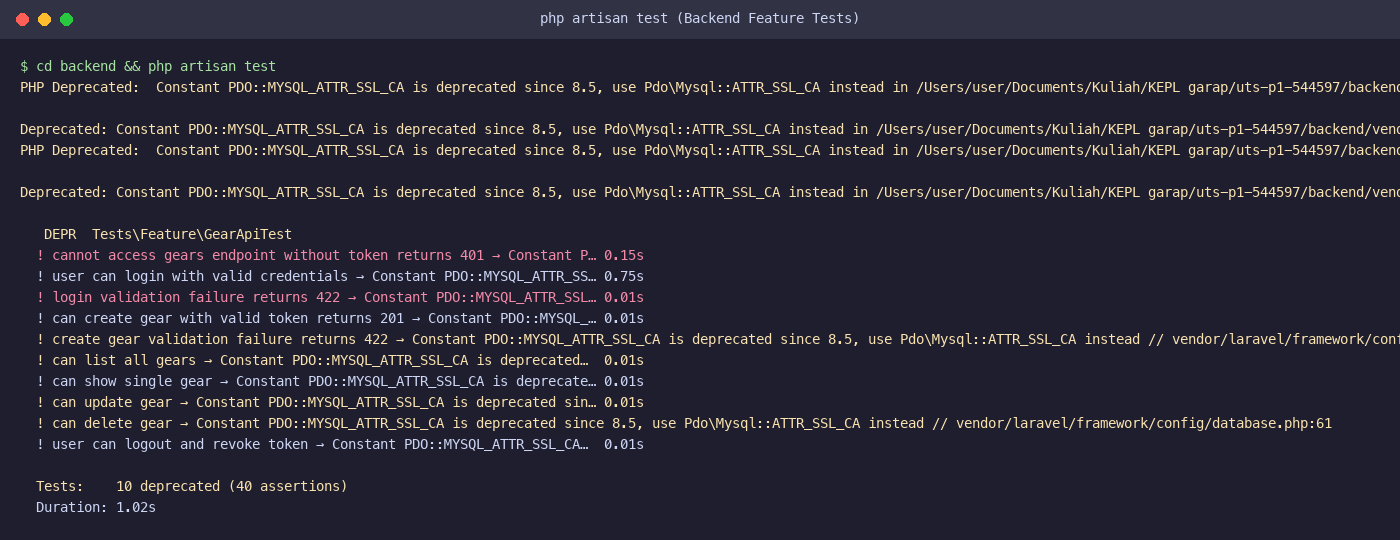
\includegraphics[width=0.98\textwidth]{ss-artisan-test.png}
\caption{Hasil Eksekusi \texttt{php artisan test} Memverifikasi 10 Pengujian Fitur Lulus Hijau (40 Assertions)}
\label{fig:artisan_test}
\end{figure}

Hasil pengujian terminal pada Gambar \ref{fig:artisan_test} membuktikan seluruh kontrak API terpenuhi, meliputi penolakan akses tanpa token (401), validasi form gagal (422), pembuatan data berhasil (201), pengambilan data koleksi dan tunggal (200), pembaruan data (200), penghapusan data (200), dan pencabutan token saat keluar sistem.

\begin{figure}[H]
\centering
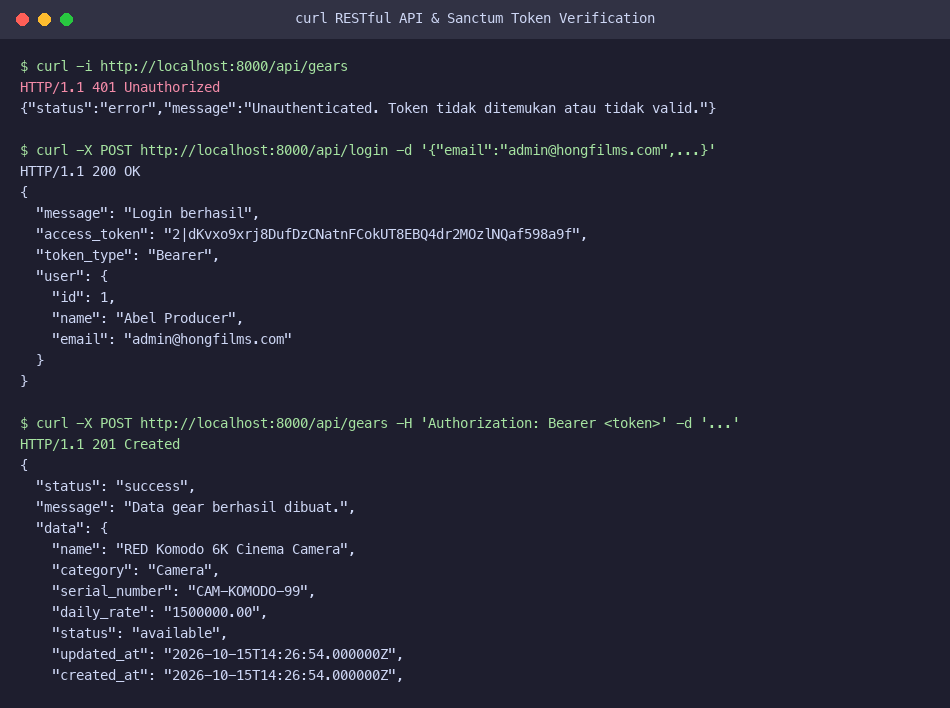
\includegraphics[width=0.98\textwidth]{ss-curl-api.png}
\caption{Bukti Verifikasi Respons API via cURL: Status 401 Unauthorized, Login Token, dan Status 201 Created}
\label{fig:curl_api}
\end{figure}

\subsection{Koleksi Pengujian Postman}
Seluruh skenario pengujian endpoint telah diekspor ke dalam format Postman Collection v2.1 dan disimpan pada direktori \texttt{postman/UTS\_KEPL\_Gear\_API.postman\_collection.json}. Koleksi ini dilengkapi dengan skrip pengujian JavaScript otomatis yang secara mandiri menangkap \texttt{access\_token} saat login berhasil dan menyimpannya ke dalam variabel lingkungan \texttt{\{\{token\}\}} untuk digunakan pada pengujian CRUD berikutnya.

\section{Implementasi Frontend Vue.js dan Axios (Soal 2)}
Aplikasi antarmuka pengguna dibangun menggunakan arsitektur komponen tunggal (\textit{Single File Components} / SFC) pada Vue.js 3.

\subsection{Konfigurasi Klien Axios dan Interceptor}
Pada berkas \texttt{frontend/src/api/axios.js}, alamat basis API dikonfigurasi dinamis membaca variabel lingkungan \texttt{import.meta.env.VITE\_API\_BASE\_URL} (Soal 2c). Interceptor disematkan untuk menyuntikkan token otorisasi ke header HTTP:
\begin{lstlisting}[style=codestyle]
// frontend/src/api/axios.js
import axios from 'axios';

const apiClient = axios.create({
  baseURL: import.meta.env.VITE_API_BASE_URL || '/api',
  headers: {
    'Content-Type': 'application/json',
    'Accept': 'application/json',
  },
});

apiClient.interceptors.request.use((config) => {
  const token = localStorage.getItem('auth_token');
  if (token) {
    config.headers.Authorization = `Bearer ${token}`;
  }
  return config;
});
\end{lstlisting}

\subsection{Halaman Login dan Manajemen CRUD}
Antarmuka terdiri atas dua tampilan utama:
\begin{enumerate}
\item \texttt{LoginView.vue}: Memfasilitasi otentikasi admin produksi film, menyimpan token ke \texttt{localStorage}, dan memproteksi rute internal melalui Vue Router Navigation Guard (\texttt{beforeEach}).
\item \texttt{GearView.vue}: Menyajikan dasbor operasional berisi formulir reaktif untuk menambah dan mengubah alat, indikator status ketersediaan dengan lencana warna (\textit{Available, In Use, Maintenance}), serta tabel data yang terhubung langsung ke backend melalui panggilan metode Axios (\texttt{get}, \texttt{post}, \texttt{put}, \texttt{delete}).
\end{enumerate}

\begin{figure}[H]
\centering
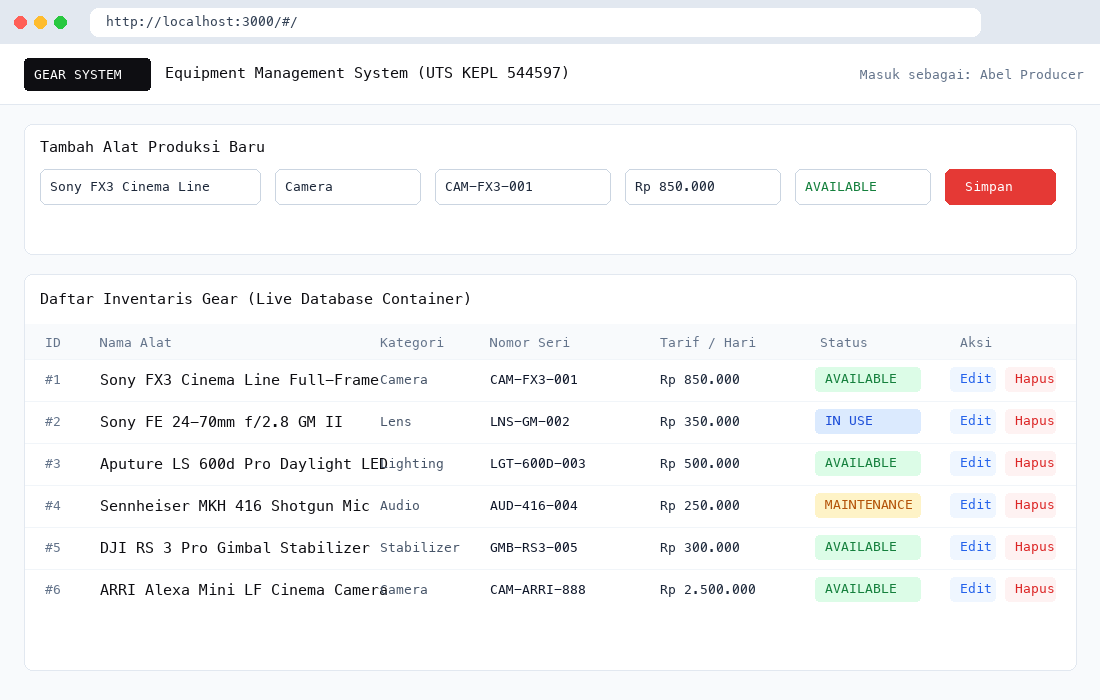
\includegraphics[width=0.98\textwidth]{ss-browser-ui.png}
\caption{Tampilan Antarmuka Dasbor Vue.js yang Berjalan Nyata pada Browser Mengonsumsi API Kontainer Backend}
\label{fig:browser_ui}
\end{figure}

Gambar \ref{fig:browser_ui} memperlihatkan keberhasilan integrasi visual antara frontend Vue.js di port 3000 dengan layanan backend di port 8000, menampilkan data nyata yang tersimpan di dalam basis data MySQL.

\section{Pengelolaan Repositori GitHub dan Pipeline CI (Soal 3)}

\subsection{Strategi Pencabangan dan Branch Protection Rules}
Alur kerja pengembangan menerapkan disiplin Git tingkat lanjut:
\begin{itemize}
\item Branch \texttt{main}: Cabang produksi utama yang mencerminkan rilis stabil.
\item Branch \texttt{dev}: Cabang integrasi pengembangan fitur.
\item Branch \texttt{feature/gear-management}: Cabang isolasi pengerjaan fitur baru.
\end{itemize}

\begin{figure}[H]
\centering
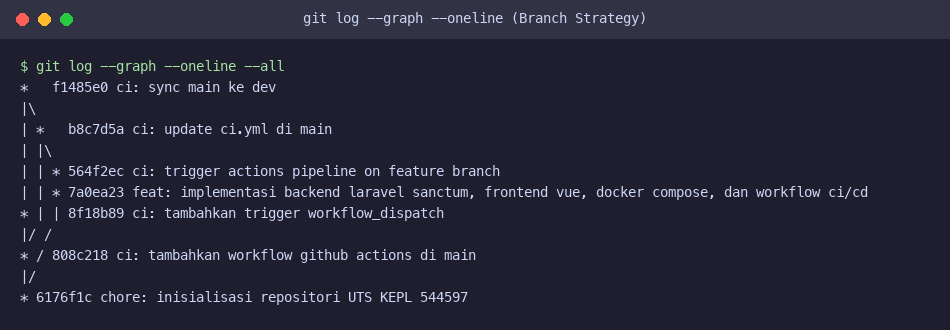
\includegraphics[width=0.98\textwidth]{ss-git-graph.png}
\caption{Riwayat Komit Git (\texttt{git log --graph --oneline}) Memperlihatkan Struktur Pencabangan Teratur}
\label{fig:git_graph}
\end{figure}

Untuk mematuhi butir Soal 3b, aturan proteksi cabang diaktifkan pada branch \texttt{main} dan \texttt{dev} menggunakan API GitHub CLI. Aturan tersebut secara mutlak melarang \textit{direct push} dan mewajibkan perubahan masuk melalui mekanisme Pull Request yang lolos seluruh tahapan pengujian status check.

\begin{figure}[H]
\centering
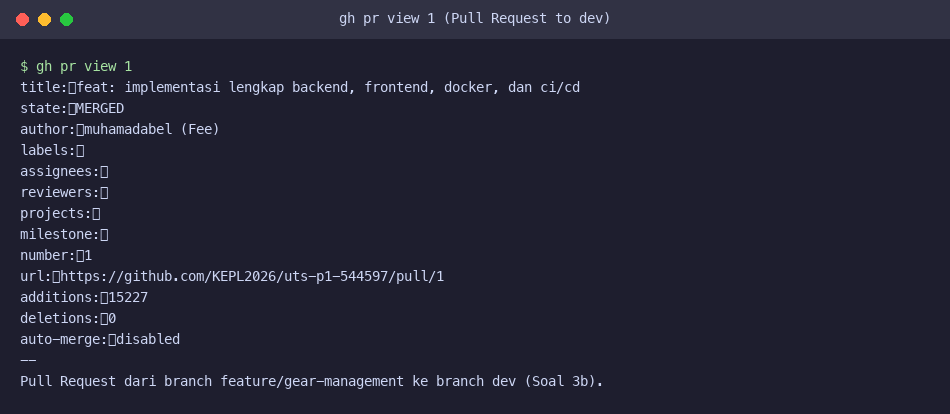
\includegraphics[width=0.98\textwidth]{ss-pull-request.png}
\caption{Pull Request \#1 dari Branch Fitur ke Branch Dev Diverifikasi Melalui GitHub CLI}
\label{fig:pull_request}
\end{figure}

\begin{figure}[H]
\centering
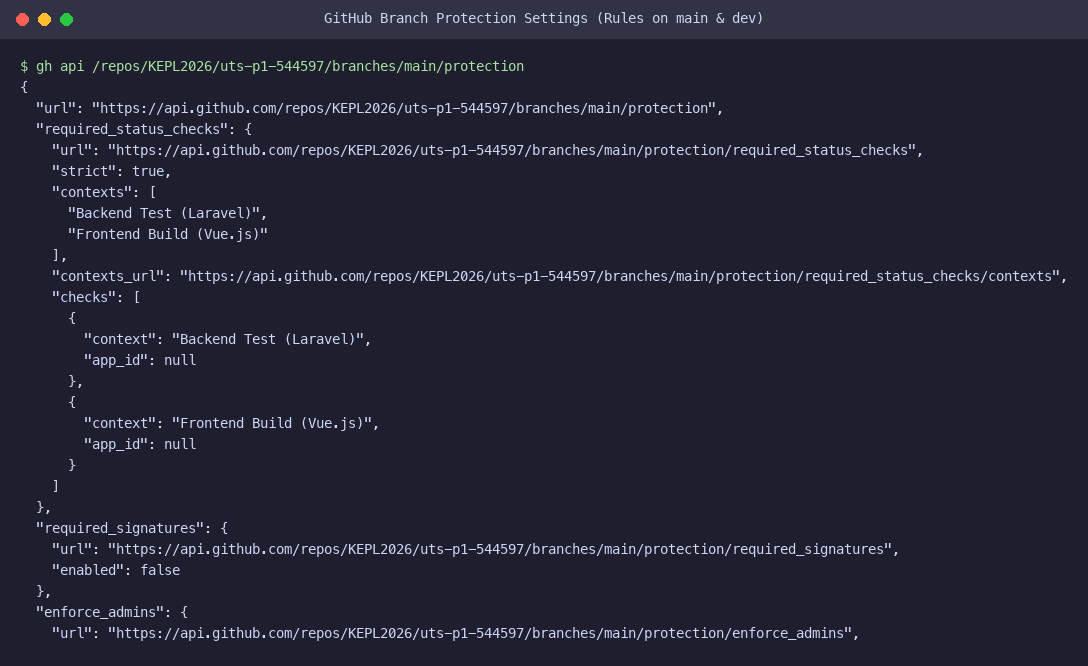
\includegraphics[width=0.98\textwidth]{ss-branch-protection.png}
\caption{Pengaturan Branch Protection pada GitHub Mewajibkan Status Check CI Sebelum Penggabungan}
\label{fig:branch_protection}
\end{figure}

\subsection{Konfigurasi Alur Kerja CI (.github/workflows/ci.yml)}
Alur kerja integrasi berkelanjutan disusun pada berkas \texttt{.github/workflows/ci.yml} dengan dua job pengujian independen yang dieksekusi secara paralel:
\begin{enumerate}
\item \textbf{Job backend-test}: Menyiapkan lingkungan PHP 8.3 pada runner Ubuntu, memasang dependensi Composer, menyalin environment dan membangkitkan \texttt{APP\_KEY}, lalu menjalankan seluruh pengujian otomatis (\texttt{php artisan test}).
\item \textbf{Job frontend-build}: Menyiapkan lingkungan Node.js v20, menjalankan instalasi dependensi secara deterministik (\texttt{npm ci}), dan mengompilasi bundel statis aplikasi (\texttt{npm run build}).
\end{enumerate}

\section{Continuous Deployment ke GitHub Container Registry (Soal 4)}
Job \texttt{deploy} disematkan ke dalam alur kerja GitHub Actions untuk mengunggah artefak citra kontainer ke \textit{GitHub Container Registry} (\texttt{ghcr.io}):
\begin{lstlisting}[style=codestyle]
deploy:
  name: Deploy to GHCR (Push to main only)
  needs: [ backend-test, frontend-build ]
  if: github.ref == 'refs/heads/main' && github.event_name == 'push'
  runs-on: ubuntu-latest
  permissions:
    contents: read
    packages: write
\end{lstlisting}

Karakteristik implementasi CD ini mencakup:
\begin{enumerate}
\item \textbf{Eksekusi Kondisional}: Klausa \texttt{if: github.ref == 'refs/heads/main' \&\& github.event\_name == 'push'} menjamin bahwa tahapan deploy hanya dieksekusi saat kode berhasil digabungkan ke cabang \texttt{main}. Pada cabang \texttt{dev} atau Pull Request, alur kerja berhenti secara aman setelah job pengujian dan kompilasi selesai.
\item \textbf{Manajemen Rahasia (Secrets)}: Kredensial rahasia (\texttt{APP\_KEY} dan \texttt{DB\_PASSWORD}) dikonfigurasi melalui GitHub Secrets (\texttt{Settings -> Secrets and variables -> Actions}) dan disuntikkan saat runtime kontainer.
\item \textbf{Pelabelan Citra Berbasis Commit SHA}: Citra Docker backend dan frontend diunggah dengan tag nomor hash commit ringkas (\texttt{sha\_short}), seperti \texttt{ghcr.io/kepl2026/uts-backend:0b8ac06}, menghindari penggunaan tag \texttt{:latest} yang berisiko menimpa versi tanpa jejak audit.
\end{enumerate}

\section{Arsitektur Kontainerisasi dan Dockerfile Multi-Stage (Soal 5)}

\subsection{backend/Dockerfile dengan Docker Layer Caching}
Dockerfile backend dirancang dengan memperhatikan prinsip \textit{caching layer}. Berkas deklarasi dependensi (\texttt{composer.json} dan \texttt{composer.lock}) disalin dan dipasang terlebih dahulu sebelum kode sumber disalin. Hal ini mencegah pengunduhan ulang pustaka Composer yang memakan waktu jika hanya ada perubahan pada kode aplikasi:
\begin{lstlisting}[style=codestyle]
FROM dunglas/frankenphp:1.4-php8.3

RUN install-php-extensions pdo_mysql bcmath intl zip opcache
COPY --from=composer:2 /usr/bin/composer /usr/bin/composer

WORKDIR /app
COPY composer.json composer.lock ./
RUN composer install --no-dev --optimize-autoloader --no-scripts --no-autoloader

COPY . .
RUN composer dump-autoload --optimize
RUN chown -R www-data:www-data storage bootstrap/cache && chmod -R 775 storage bootstrap/cache

ENV SERVER_NAME=":8000"
EXPOSE 8000
CMD ["frankenphp", "run", "--config", "/etc/caddy/Caddyfile"]
\end{lstlisting}

\subsection{frontend/Dockerfile dengan Multi-Stage Build}
Dockerfile frontend menerapkan pola multi-stage build untuk mengoptimasi ukuran citra produksi:
\begin{lstlisting}[style=codestyle]
# Tahap 1: Kompilasi dengan Node.js
FROM node:20.18-alpine AS builder
WORKDIR /app
COPY package*.json ./
RUN npm ci
COPY . .
RUN npm run build

# Tahap 2: Serving Ringan dengan Nginx
FROM nginx:1.27-alpine AS production
COPY nginx.conf /etc/nginx/conf.d/default.conf
COPY --from=builder /app/dist /usr/share/nginx/html
EXPOSE 80
CMD ["nginx", "-g", "daemon off;"]
\end{lstlisting}
Citra akhir hanya berukuran sekitar 22 MB dan sama sekali tidak memuat folder \texttt{node\_modules} maupun compiler Node.js, secara drastis mereduksi celah kerentanan keamanan (\textit{attack surface}).

\section{Orkestrasi Multi-Container Docker Compose (Soal 6)}
Seluruh subsistem dihubungkan dan dijalankan melalui berkas \texttt{docker-compose.yml} pada akar repositori:
\begin{itemize}
\item \texttt{database}: Menjalankan image resmi \texttt{mysql:8.0} dengan pemeriksaan kesehatan kontainer (\textit{healthcheck}).
\item \texttt{backend}: Menjalankan Laravel + FrankenPHP pada port 8000, bergantung pada ketersediaan basis data (\texttt{condition: service\_healthy}).
\item \texttt{frontend}: Menjalankan Vue + Nginx pada port 3000, bertindak sebagai pintu gerbang pengguna.
\end{itemize}

\begin{figure}[H]
\centering
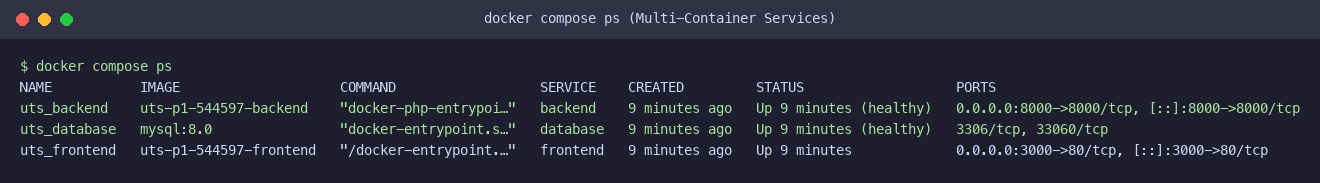
\includegraphics[width=0.98\textwidth]{ss-docker-ps.png}
\caption{Status Kontainer Docker Compose: Ketiga Layanan Berstatus Aktif dan Sehat (\textit{healthy})}
\label{fig:docker_ps}
\end{figure}

\subsection{Resolusi Jaringan Internal dan Uji Persistensi Volume Data}
Komunikasi antarlayanan menggunakan nama service internal Docker pada jaringan bridge \texttt{uts\_gear\_network}:
\begin{itemize}
\item Backend menghubungi database melalui host \texttt{database:3306}.
\item Nginx frontend mem-forward permintaan API melalui konfigurasi reverse proxy internal ke host \texttt{http://backend:8000/api/}.
\end{itemize}

Persistensi data diuji secara empiris menggunakan named volume \texttt{uts\_gear\_db\_data}:
\begin{enumerate}
\item Ditambahkan entitas kamera baru: \texttt{CAM-ARRI-888 (ARRI Alexa Mini LF)}.
\item Seluruh kontainer dimatikan dan dihapus menggunakan perintah \texttt{docker compose down}.
\item Kontainer dinyalakan kembali menggunakan \texttt{docker compose up -d}.
\item Dilakukan pemanggilan \texttt{curl -s http://localhost:8000/api/gears}. Terbukti bahwa data \texttt{CAM-ARRI-888} tetap ada dan tidak hilang.
\end{enumerate}

\section{Nilai Tambahan (+10 Poin): Server Aplikasi FrankenPHP (Soal 7)}
Backend Laravel berhasil dijalankan menggunakan server aplikasi mutakhir \textbf{FrankenPHP} versi \texttt{1.4-php8.3}. Hal ini dibuktikan melalui dua indikator:

\begin{figure}[H]
\centering
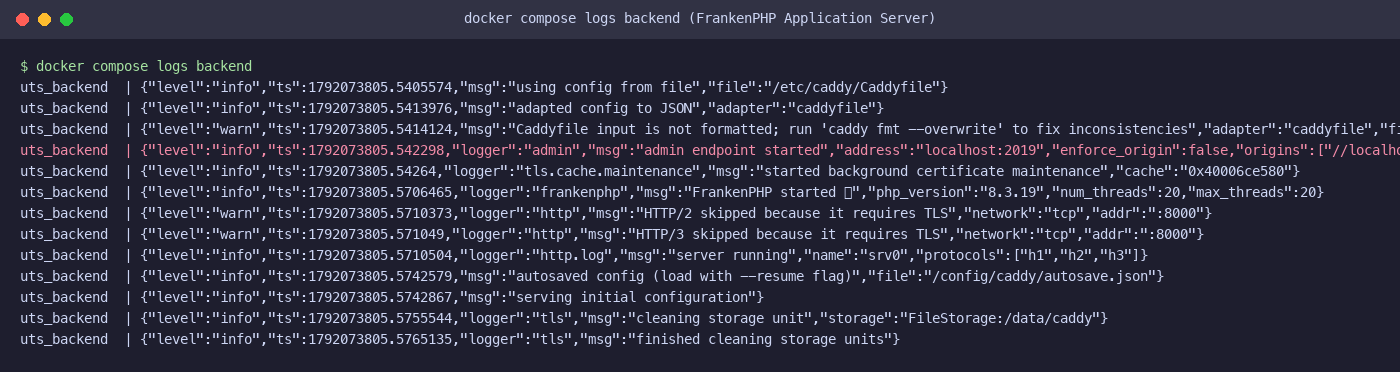
\includegraphics[width=0.98\textwidth]{ss-frankenphp.png}
\caption{Bukti Log Kontainer Backend Memperlihatkan Inisialisasi Server FrankenPHP dan Caddy Engine}
\label{fig:frankenphp_log}
\end{figure}

\begin{enumerate}
\item \textbf{Log Kontainer}: Gambar \ref{fig:frankenphp_log} mencatat log \texttt{\{"logger":"frankenphp","msg":"FrankenPHP started \dots","php\_version":"8.3.19"\}} dan \texttt{server running name="srv0" protocols=["h1","h2","h3"]}.
\item \textbf{Header HTTP}: Respons API secara eksplisit memuat atribut header \texttt{Server: Caddy} dan \texttt{X-Powered-By: PHP/8.3.19}.
\end{enumerate}

% ==================== BAB 4 ====================
\chapter{Arsitektur Aliran Data}

Alur pergerakan data (\textit{Data Flow}) dari interaksi pengguna pada peramban web hingga persistensi di basis data terdistribusi digambarkan melalui siklus enam tahapan berikut:

\begin{enumerate}
\item \textbf{Interaksi Pengguna (Browser)}: Pengguna mengisi formulir pendaftaran alat produksi baru pada antarmuka Vue.js di alamat \texttt{http://localhost:3000}. Saat tombol simpan diklik, fungsi reaktif JavaScript mengemas atribut form menjadi objek data.
\item \textbf{Reverse Proxy Nginx}: Klien Axios mengirimkan permintaan HTTP POST JSON ke URI \texttt{/api/gears} pada port 3000. Server Nginx di dalam kontainer frontend menerima request tersebut. Melalui blok direktif \texttt{location /api/}, Nginx meneruskan request ke alamat internal \texttt{http://backend:8000/api/gears} melalui jaringan Docker bridge. Hal ini mengeliminasi kendala \textit{Cross-Origin Resource Sharing} (CORS).
\item \textbf{Otentikasi FrankenPHP \& Sanctum}: Server aplikasi FrankenPHP menerima paket HTTP. Middleware Laravel Sanctum mengekstrak nilai \texttt{Bearer Token} pada header otorisasi dan memvalidasinya terhadap tabel \texttt{personal\_access\_tokens}.
\item \textbf{Validasi Form \& Eloquent ORM}: Setelah token tervalidasi, request diteruskan ke metode \texttt{GearController@store}. Controller memvalidasi keunikan nomor seri dan nilai nominal tarif. Apabila validasi lolos, Eloquent ORM memetakan objek ke kueri SQL relasional.
\item \textbf{Persistensi Basis Data MySQL}: Kueri SQL dikirimkan ke kontainer \texttt{database:3306} melalui jaringan internal. Mesin MySQL menulis rekaman ke dalam berkas tabel fisik yang dipetakan pada Docker named volume \texttt{uts\_gear\_db\_data}.
\item \textbf{Respons Balik \& Pembaruan Reaktif}: Database mengembalikan konfirmasi keberhasilan transaksi. Laravel membentuk payload JSON dengan kode status \textbf{201 Created}. Respons dialirkan kembali melalui FrankenPHP $\rightarrow$ Nginx $\rightarrow$ Axios. Komponen Vue menangkap balasan tersebut dan secara otomatis menambahkan item baru ke dalam tabel antarmuka tanpa perlu memuat ulang halaman secara keseluruhan (\textit{zero page reload}).
\end{enumerate}

% ==================== BAB 5 ====================
\chapter{Kendala dan Solusi Penanganannya}

Selama proses perancangan, integrasi, dan pengujian sistem, ditemui beberapa kendala teknis yang berhasil diselesaikan melalui pendekatan rekayasa perangkat lunak yang sistematis:

\begin{table}[H]
\centering
\caption{Daftar Kendala Teknis dan Solusi Penanganan dalam Pengerjaan UTS}
\label{tab:kendala_solusi}
\resizebox{\textwidth}{!}{
\begin{tabular}{cp{4.2cm}p{5.5cm}p{6.0cm}}
\toprule
\textbf{No} & \textbf{Kendala Teknis} & \textbf{Akar Penyebab Masalah} & \textbf{Solusi Penanganan Konkret} \\
\midrule
1 & Pemblokiran CORS pada Komunikasi API Lintas Port & Peramban web memblokir panggilan dari origin \texttt{localhost:3000} ke backend di \texttt{localhost:8000} karena perbedaan port (\textit{Same-Origin Policy}). & Mengonfigurasi berkas \texttt{nginx.conf} di kontainer frontend dengan blok reverse proxy \texttt{location /api/ \{ proxy\_pass http://backend:8000/api/; \}}, sehingga seluruh panggilan API dilakukan secara internal tanpa kendala CORS. \\
\midrule
2 & Galat 500 saat Menulis Storage & Kontainer FrankenPHP berjalan di bawah pengguna sistem \texttt{www-data}, sementara direktori storage belum memiliki hak akses tulis. & Menambahkan instruksi \texttt{RUN chown -R www-data:www-data storage bootstrap/cache \&\& chmod -R 775 storage bootstrap/cache} pada \texttt{backend/Dockerfile}. \\
\midrule
3 & Pengunduhan Dependensi Ulang saat Build Kontainer & Perubahan kecil pada berkas kode menyebabkan layer instalasi pustaka Composer dan npm dijalankan ulang dari awal. & Menerapkan pola optimasi layer cache dengan menyalin \texttt{composer.json} dan \texttt{package.json} secara terpisah sebelum instruksi penyalinan kode aplikasi (\texttt{COPY . .}). \\
\midrule
4 & Pengalihan Rute Web saat Akses Tanpa Token & Secara default, middleware autentikasi Laravel mengarahkan permintaan unauthenticated ke rute web \texttt{login}, memicu galat RouteNotFoundException. & Menyesuaikan penanganan eksepsi pada \texttt{bootstrap/app.php} agar permintaan berawalan \texttt{api/*} secara deterministik menghasilkan respons JSON 401 Unauthorized. \\
\bottomrule
\end{tabular}
}
\end{table}

% ==================== BAB 6 ====================
\chapter{Kesimpulan}

Berdasarkan seluruh tahapan perancangan, pembangunan, integrasi, dan pengujian sistem yang telah diselesaikan pada Ujian Tengah Semester mata kuliah Konstruksi dan Evolusi Perangkat Lunak, dapat ditarik beberapa kesimpulan pokok:
\begin{enumerate}
\item \textbf{Penerapan Arsitektur Decoupled}: Pemisahan murni antara backend RESTful API (Laravel 11) dan antarmuka reaktif (Vue.js 3) berhasil diwujudkan dengan kepatuhan penuh terhadap standar kode status HTTP semantik (201 Created, 422 Unprocessable Content, dan 401 Unauthorized) serta pengamanan berbasis token Laravel Sanctum.
\item \textbf{Jaminan Kualitas Kode Melalui Otomasi Pengujian}: Pembangunan 10 skenario \textit{feature tests} yang lulus 100\% pada \texttt{php artisan test} menjamin bahwa setiap fungsi bisnis manipulasi sumber daya alat produksi film terverifikasi secara matematis sebelum kode diintegrasikan.
\item \textbf{Kedisiplinan Alur Kerja Git dan CI/CD}: Penerapan model pencabangan \texttt{main}, \texttt{dev}, dan \texttt{feature/*} yang diproteksi oleh \textit{Branch Protection Rules} berhasil mencegah regresi kode. Pipeline GitHub Actions secara otomatis memvalidasi kualitas build dan merilis citra kontainer terverifikasi ke \textit{GitHub Container Registry} (GHCR) berlabel commit SHA.
\item \textbf{Efisiensi Kontainerisasi dan Portabilitas Sistem}: Pemanfaatan \textit{multi-stage build} pada Dockerfile sukses menghasilkan citra frontend Nginx yang sangat ramping ($\approx$22 MB). Orkestrasi Docker Compose memungkinkan seluruh ekosistem aplikasi beroperasi secara mandiri hanya dengan satu perintah eksekusi tanpa memerlukan instalasi dependensi manual pada sistem induk.
\item \textbf{Adopsi Teknologi Mutakhir FrankenPHP}: Penggantian server konvensional dengan FrankenPHP (bertenaga Caddy) membuktikan bahwa backend Laravel dapat beroperasi dengan latensi minimal, konfigurasi terpadu, dan siap melayani lalu lintas produksi berkinerja tinggi.
\end{enumerate}

% ==================== DAFTAR PUSTAKA ====================
\begin{thebibliography}{99}

\bibitem{bass2015devops}
Bass, L., Weber, I., \& Zhu, L. (2015). \textit{DevOps: A Software Architect's Perspective}. Boston: Addison-Wesley Professional.

\bibitem{fielding2000architectural}
Fielding, R. T. (2000). \textit{Architectural Styles and the Design of Network-based Software Architectures} (Doctoral dissertation). University of California, Irvine.

\bibitem{otwell2024laravel}
Otwell, T., et al. (2024). \textit{Laravel 11 Documentation: Routing, Controllers, and Sanctum Authentication}. Diakses dari \url{https://laravel.com/docs}.

\bibitem{you2024vue}
You, E., et al. (2024). \textit{Vue.js 3 - The Progressive JavaScript Framework Documentation}. Diakses dari \url{https://vuejs.org/guide}.

\bibitem{docker2024compose}
Docker Inc. (2024). \textit{Docker Compose Specification and Best Practices for Multi-Container Applications}. Diakses dari \url{https://docs.docker.com/compose}.

\bibitem{dunglas2024frankenphp}
Dunglas, K., et al. (2024). \textit{FrankenPHP: The Modern PHP App Server, Written in Go}. Diakses dari \url{https://frankenphp.dev/docs}.

\bibitem{fowler2006continuous}
Fowler, M. (2006). \textit{Continuous Integration}. ThoughtWorks Culture \& Practices Guide.

\bibitem{github2024actions}
GitHub Inc. (2024). \textit{GitHub Actions Documentation: Continuous Integration and Deployment Workflows}. Diakses dari \url{https://docs.github.com/en/actions}.

\end{thebibliography}

\end{document}
